\documentclass[12pt,letterpaper,titlepage,en-US]{article}

\usepackage{basicstyle}
\usepackage{report}
%\usepackage{knit}

\usepackage{listings}
\usepackage{xcolor}


\definecolor{codegreen}{rgb}{0,0.6,0}
\definecolor{codegray}{rgb}{0.5,0.5,0.5}
\definecolor{codepurple}{rgb}{0.58,0,0.82}
\definecolor{backcolour}{rgb}{0.95,0.95,0.92}
 
\lstdefinestyle{mystyle}{
    backgroundcolor=\color{backcolour},   
    commentstyle=\color{codegreen},
    keywordstyle=\color{magenta},
    numberstyle=\tiny\color{codegray},
    stringstyle=\color{codepurple},
    basicstyle=\ttfamily\footnotesize,
    breakatwhitespace=false,         
    breaklines=true,                 
    captionpos=b,                    
    keepspaces=true,                 
    numbers=left,                    
    numbersep=5pt,                  
    showspaces=false,                
    showstringspaces=false,
    showtabs=false,                  
    tabsize=2
}
 
\lstset{style=mystyle}



\usepackage[toc,page]{appendix}

\newcommand{\hmwkTitle}{Project \#3}
\DTMsavetimestamp{DueDate}{2019-11-27T11:59:00+00:00}
\newcommand{\hmwkClass}{CS 6385.001}
\newcommand{\hmwkClassName}{Algorithmic Aspects of Telecommunication Networks}
\newcommand{\hmwkClassInstructor}{Instructor: Prof. Andras Farago}
\newcommand{\hmwkAuthorName}{Shyam Patharla}
\newcommand{\hmwkAuthorNetID}{sxp178231}




%
% Title Page
%

\title{
    \vspace{1in}
    \textmd{\textbf{\hmwkClassName \\\hmwkClass:\ \hmwkTitle }}\\
    \normalsize\vspace{0.1in}\small{Due\ on\ \DTMusedate{DueDate}\ at \DTMusetime{DueDate} }\\
    \vspace{0.1in}\large{\textit{\hmwkClassInstructor}}\\
    \vspace{0.5in}
\includegraphics[height=2.4em]{UTD_logo_BW}\\
    \vspace{2in}
}

\author{\textbf{\hmwkAuthorName\ \footnotesize{(\hmwkAuthorNetID)}} \\ }
\date{}
\makeindex

\begin{document}
\maketitle
\pagenumbering{Roman}

\tableofcontents

\pagebreak
\pagenumbering{arabic}

\section{Introduction}
\begin{itemize}
\item In this project, we try to implement the Exhaustive Enumeration   algorithm for finding the reliability of a network
\item Give an input network with n nodes , m edges, and component reliability p, our program outputs the reliability of the network 
\item We do this for range of values of p
\item We can also flip the system condition for k states
\item  We also analyze how the reliability varies with the value of k when the value of p is fixed
\item We discuss the possible reasons for the above characteristics.
\end{itemize}

\section{Design Decisions}
\begin{itemize}
\item We implement the solution in the \textbf{Java} programming language
\item We use the \textbf{Eclipse} IDE since it has a lot of help for debugging 
\item The program modules were run on a \textbf{Mac} operating system

\end{itemize}





\section{Solution Approach}

\subsection{Generating Input Examples}
We first generate  input graphs for simulating the algorithm.
These graphs are then passed on to \textit{Module 2}  which runs the Exhaustive Enumeration algorithm on them. The graphs are generated as follows.

\begin{itemize}
\item For all examples, we set the number of nodes in the network to 5 i.e \textit{n} = 5

\item The topology of the graph for all examples is a complete graph, hence the number of edges m=10



\end{itemize}




\subsection{Exhaustive Enumeration Algorithm}
\textit{Module 2} receives input parameters from the first module (graph). It has the following functions.


\begin{itemize}
\item The \textbf{n} nodes in our network are always up
\item We have \textbf{m} links each of which may fail
\item The minimum number of links that may fail in a particular state is \textbf{zero}, while the maximum number is \textbf{m}
\item We can generate \textbf{$2^{m}$} possible states, each of which may contain some links which fail and some links do not
\item We proceed step by step, generating states with \textbf{k} failures, k=0,1,2,...m and store them

\end{itemize}

Module 2  passes the generated states it on to Module 3, which computes the raliability for the network.



\subsection{Reliability}

\textit{Module 3} takes the output parameters of \textit{Module 2} i.e. the \textbf{generated states} for an input network

\begin{itemize}


\item We iterate through the states received

 \item For each state we check if the network is \textit{connected} using a \textbf{depth first search}
 
 \item  If it is connected, then the system condition is \textbf{up}, else the system condition is \textit{down}

\item We compute the \textbf{probability} of the state \textit{s} using the formula
\begin{equation}
prob(s)=p*u + (1-p)*d
\end{equation}

where \textbf{u} is the number of links which are up and \textbf{d} is the number of links which are down

\item The \textbf{reliability} of the network is the sum of probabilities of the \textbf{up} states
 
\end{itemize}


\subsection{Presentation of Results}
\begin{itemize}

\item We use a value \textbf{p} to denote the reliability of a component (link) 

\item We also use a parameter \textbf{k} which denotes the number of states (randomly chosen) whose condition is flipped i.e. from up to down or vice versa

\item \textit{Task 1} consists of varying the value of \textbf{p} and seeing how the reliability of the network changes

\item We vary the value of p  from 0 to 1 in steps of 0.04  

 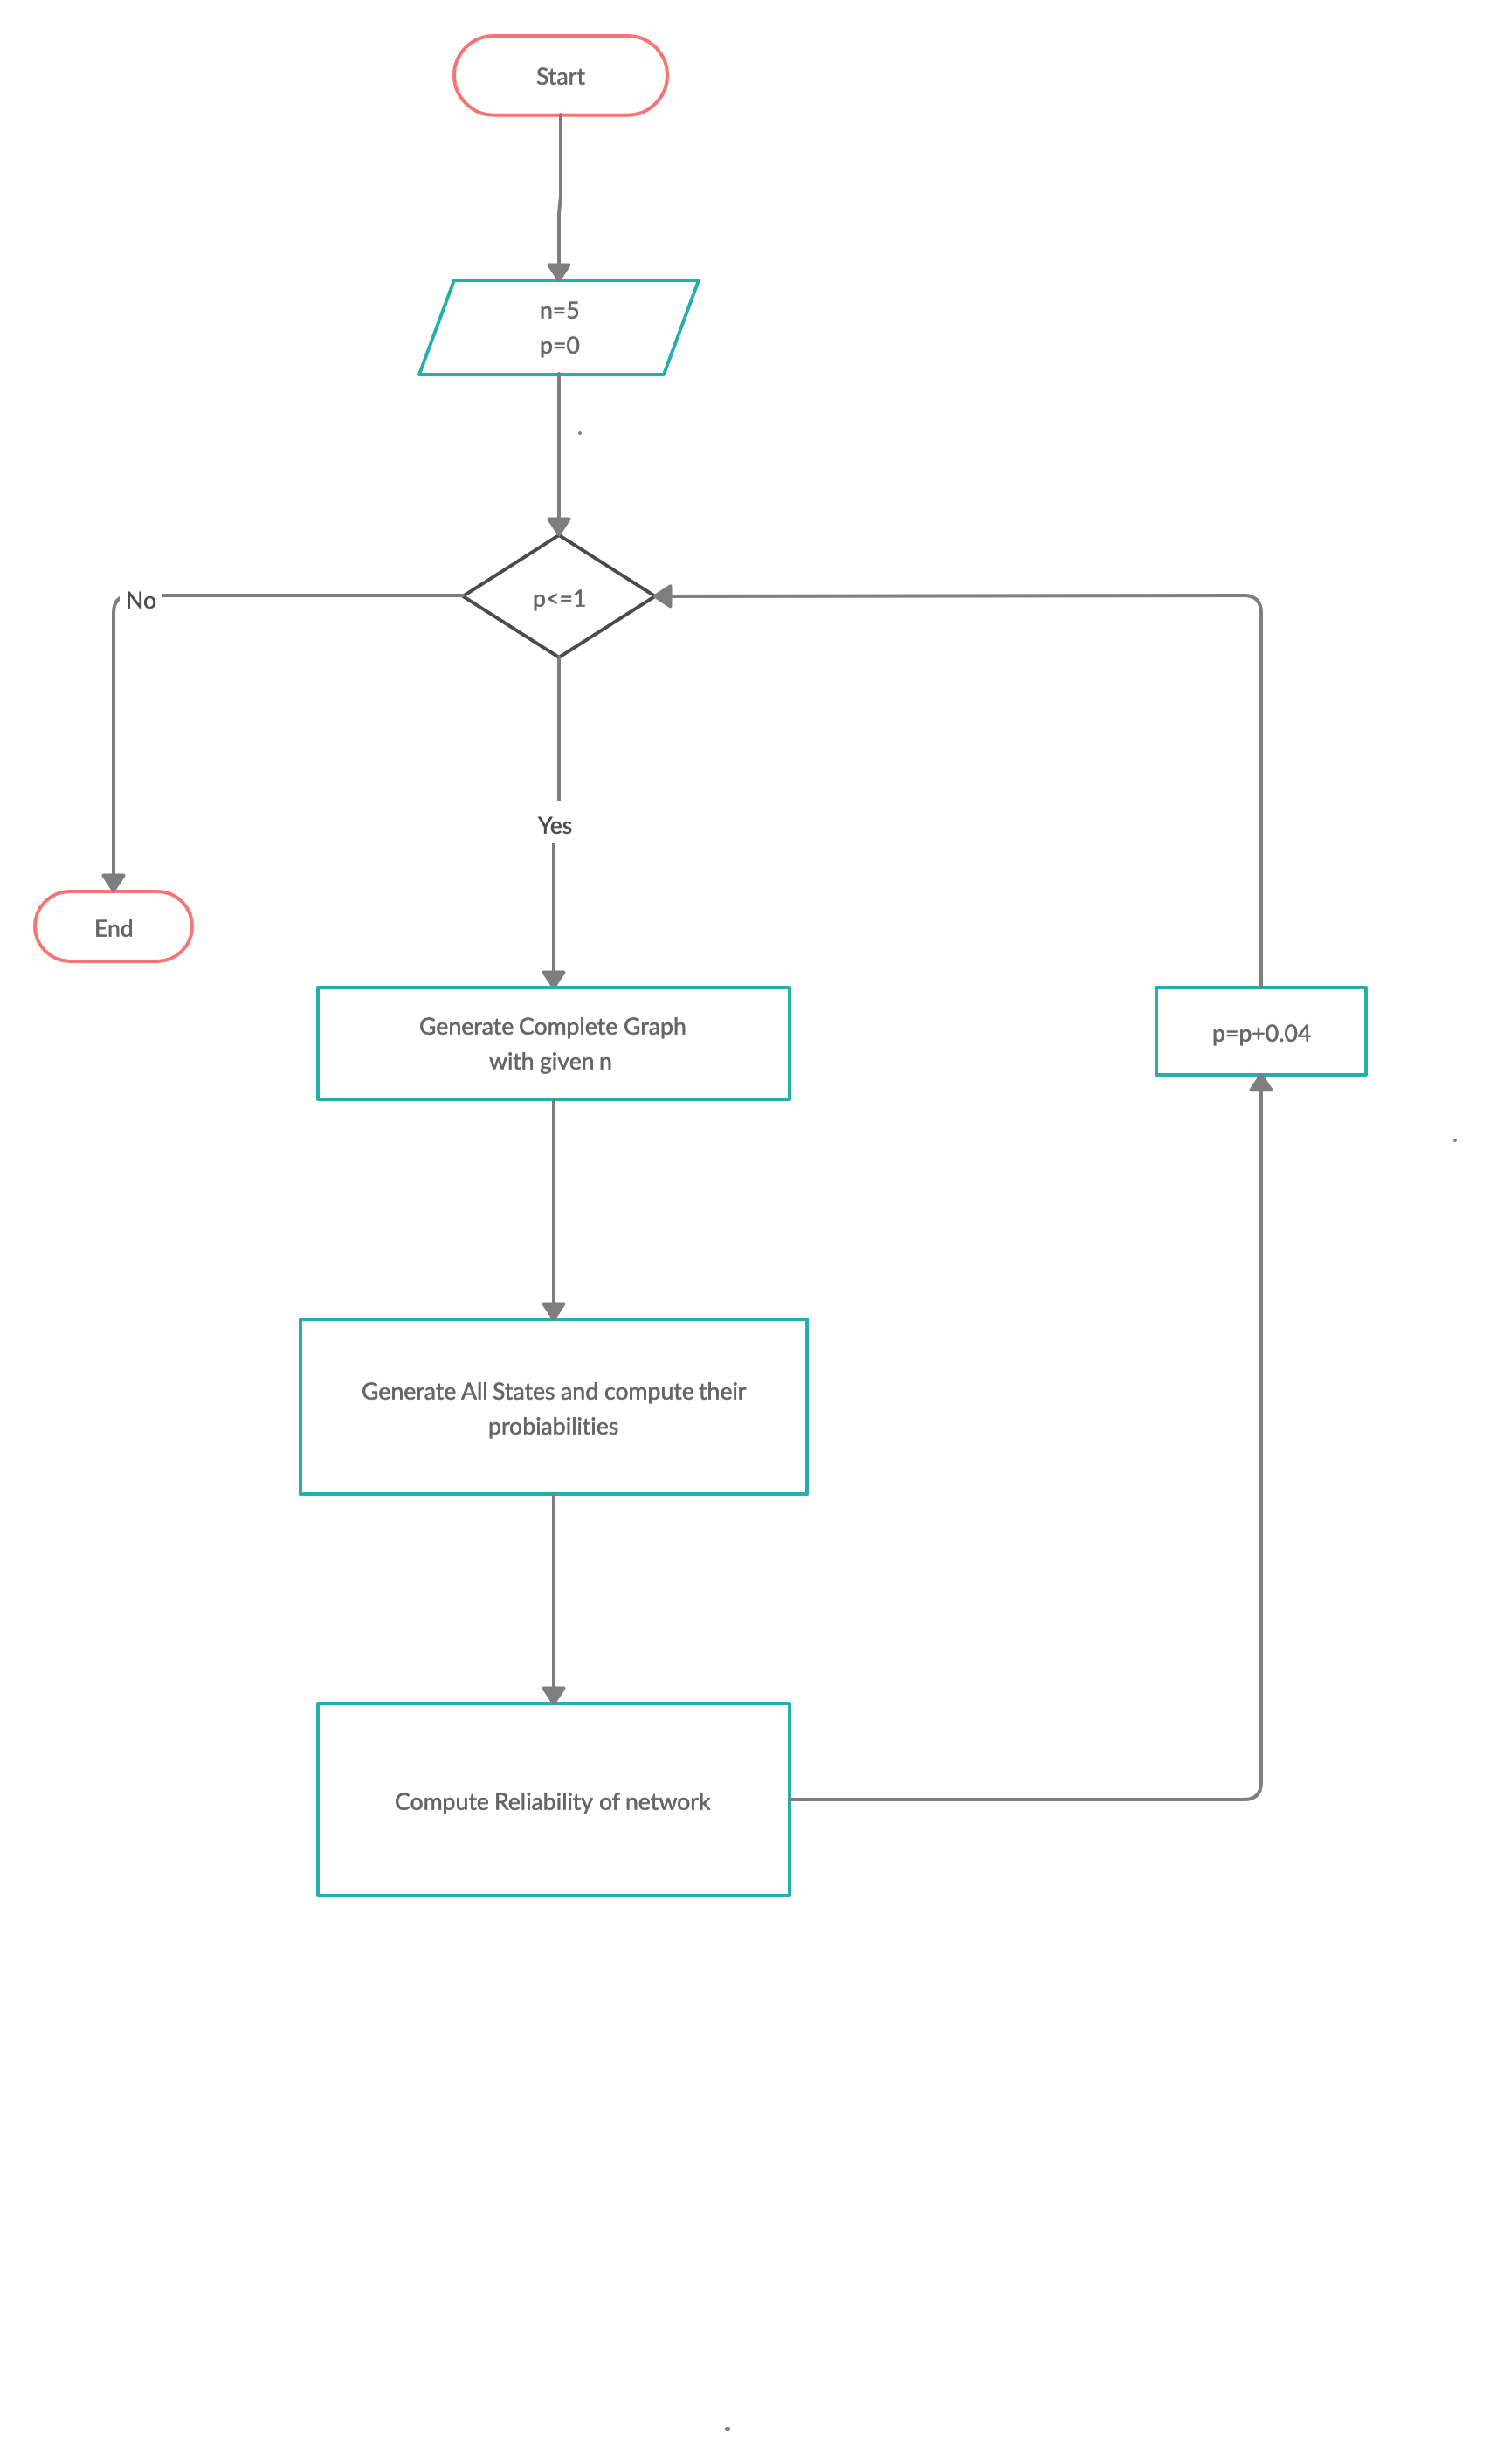
\includegraphics[scale=0.20]{fig/task1.png}
 
 

\item \textit{Task 2} consists of fixing the value of \textbf{p}, varying \textbf{k} and seeing how the reliability of the network varies

\item We fix the value of p to 0.87 and vary the value of k from 0 to 25 in steps of 1 

\item We take 5 trials for each value of k and take the average of the reliabilities
 \end{itemize}

The flowchart for Task 2 is shown below.

 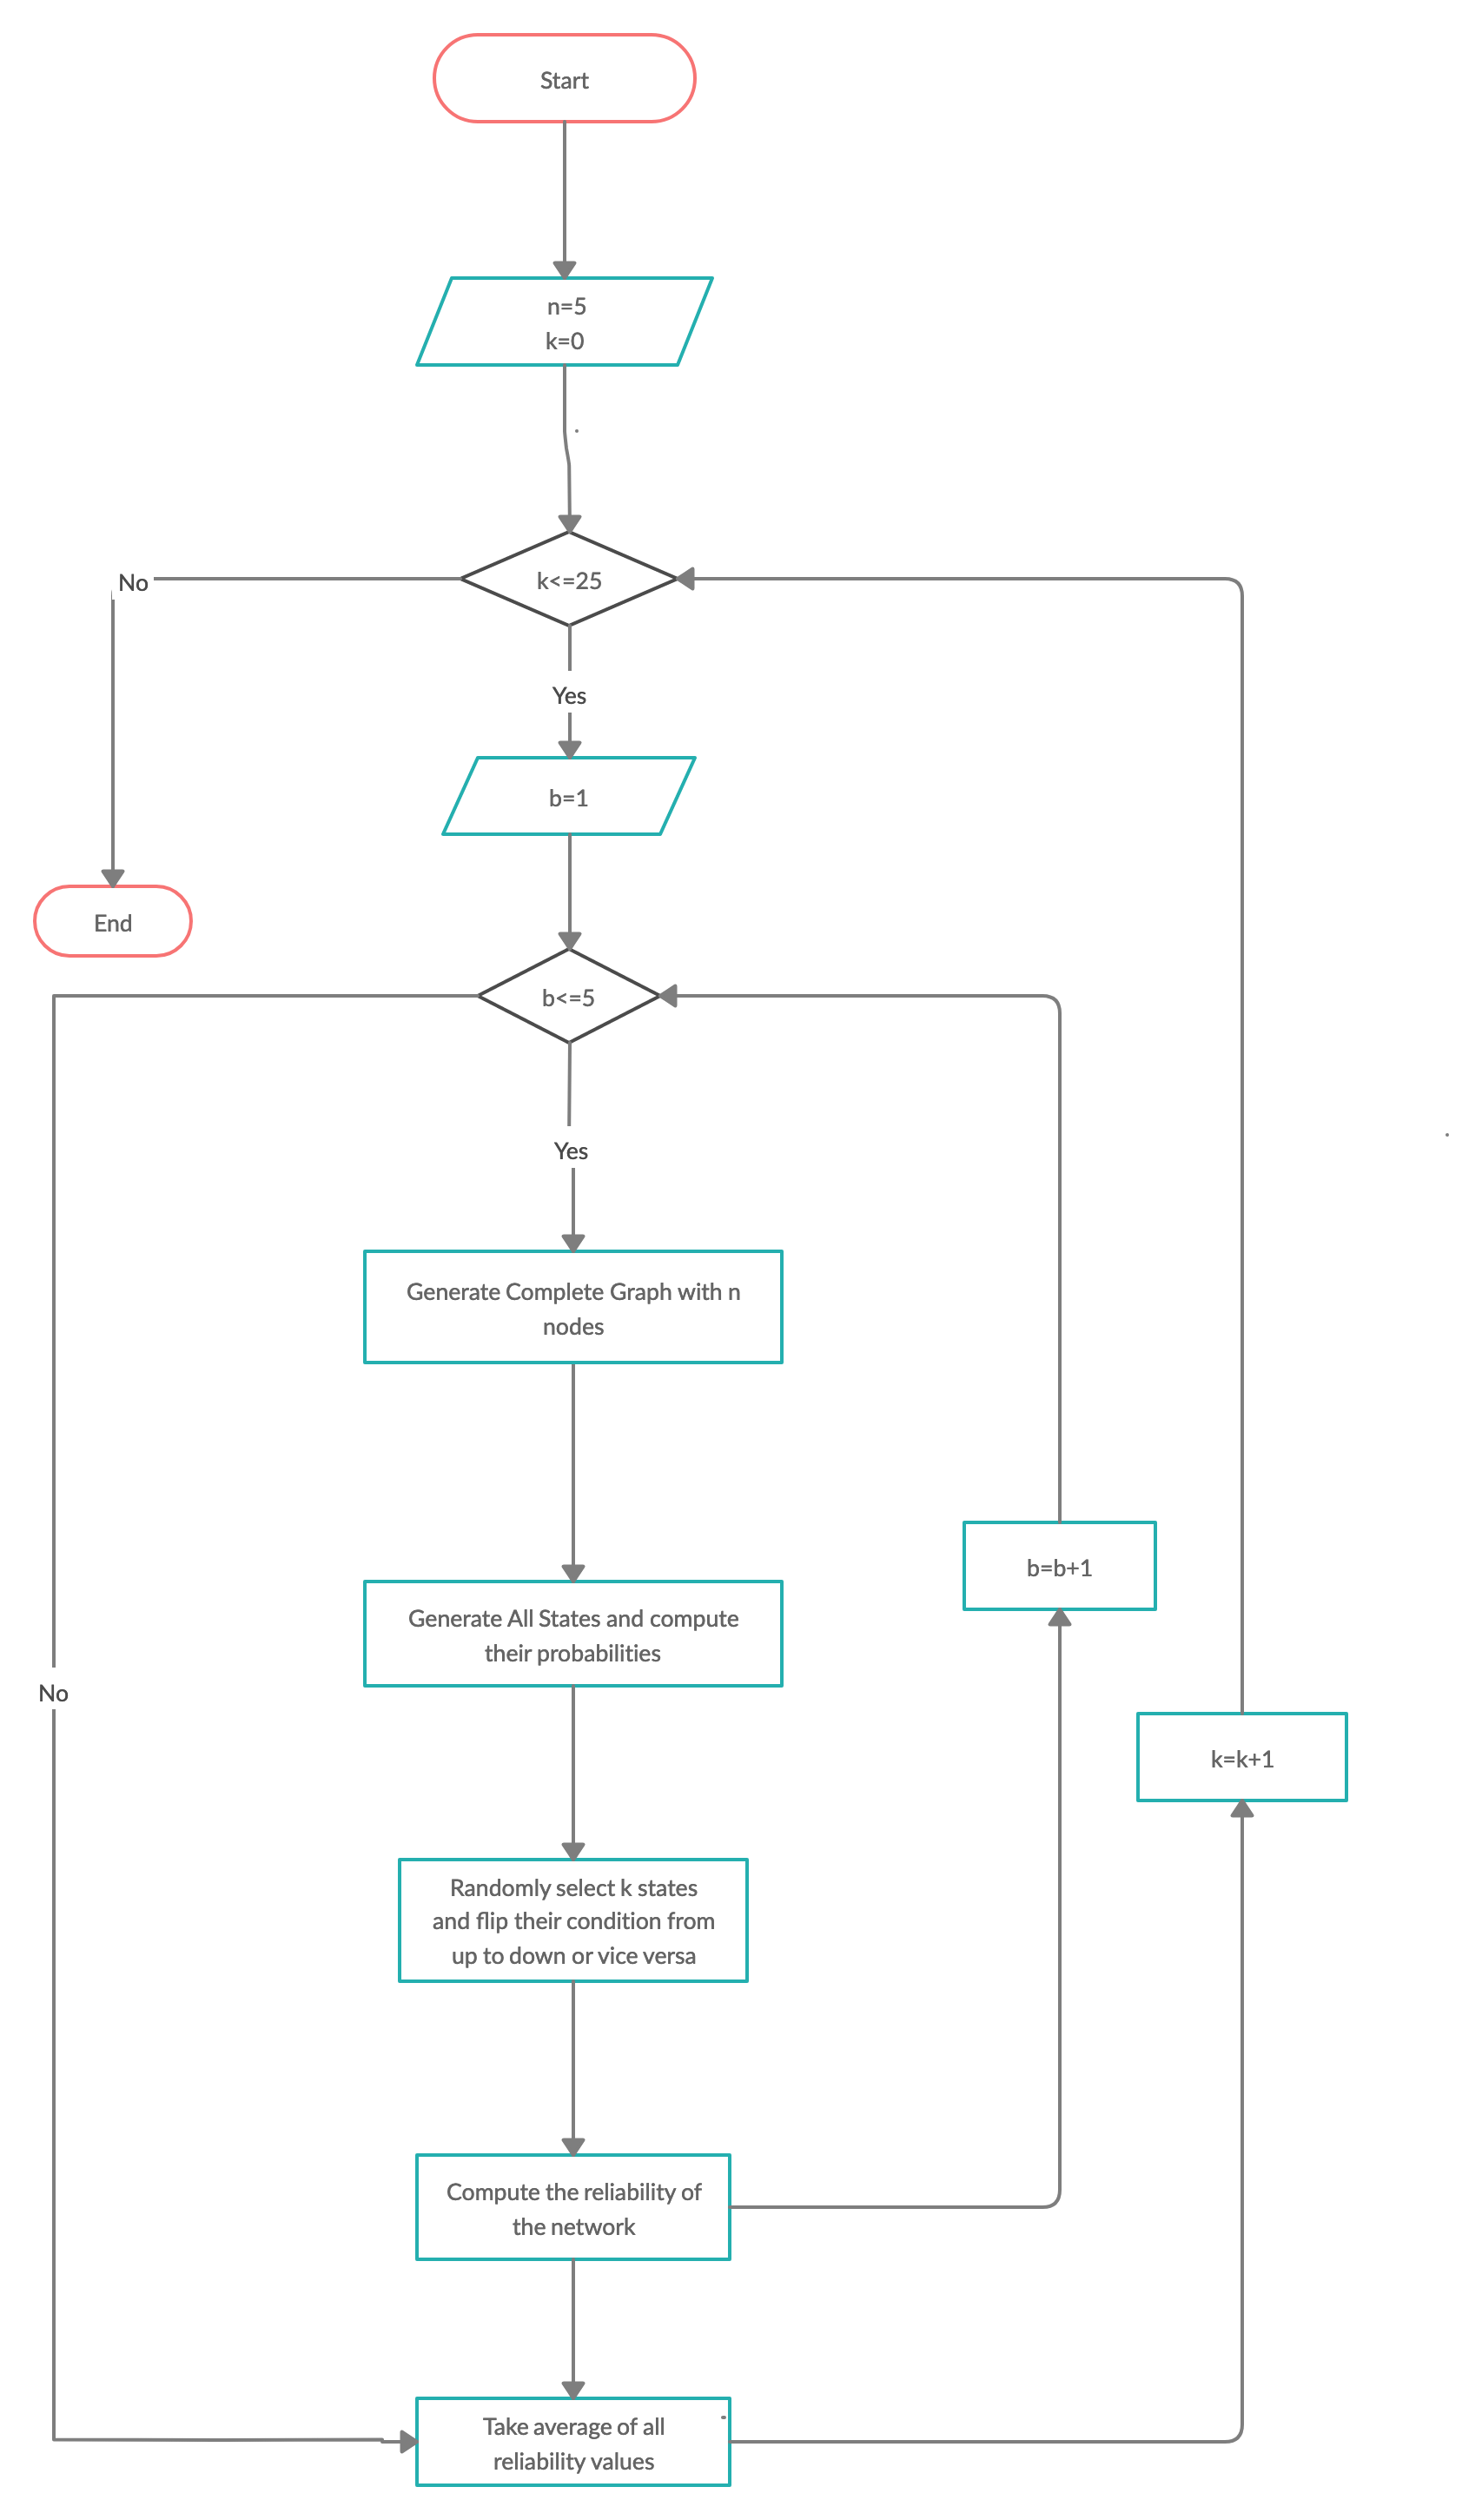
\includegraphics[scale=0.20]{fig/task2.png}


\section{Exhaustive Enumeration Algorithm - Explanation}
\begin{itemize}


\item The goal is to find the \textit{reliability} of a network where nodes are always up but links may fail

\item We generate \textbf{all possible states} for the network where each component may be \textit{up} or \textit{down}

\item For each state, we check if the network is \textbf{connected}

\item If it is connected we compute its probability using the formula
\begin{equation}
prob(s)=p*u + (1-p)*d
\end{equation}

where \textbf{u} is the number of links which are up and \textbf{d} is the number of links which are down


\item The \textbf{reliability} of the network is the sum of probabilities of all \textit{up} states





\end{itemize}








\begin{algorithm}[H]
    \caption{ExhaustiveEnumeration}
    \begin{algorithmic}[1]
        \Procedure{ExhaustiveEnumeration}{$V,E,p$}
      
      \State $m= \mid E \mid$
      \State $states[][] = generateStates(m)$
      
      \State $t = 2^m $
     \State $reliability=0$
      
      
      \For {$i = 1 \text{ to } t$}
      	
      	\State $ s = states[i]$
      	\State $fail=0$
      	
      	\For {$j=1 \text{ to } m$}
      		\If {$s[j]=1$}
      			\State $fail=fail+1$
      			\EndIf
      			\EndFor
      			
      	\State $prob=p*(m-fail)+(1-p)*fail$
      	\State $G' = transform(V,E,s)$
      	\If {$isConnected(G')$}
      	\State $reliability=reliability+prob$
      	\EndIf
      	
      	
      \EndFor
      
        
      
     
     
      return reliability
        \EndProcedure
    \end{algorithmic}
    \end{algorithm}




\section{Observations and Analysis}
\begin{itemize}


\item The program produces outputs as shown in the figures below.\\
 
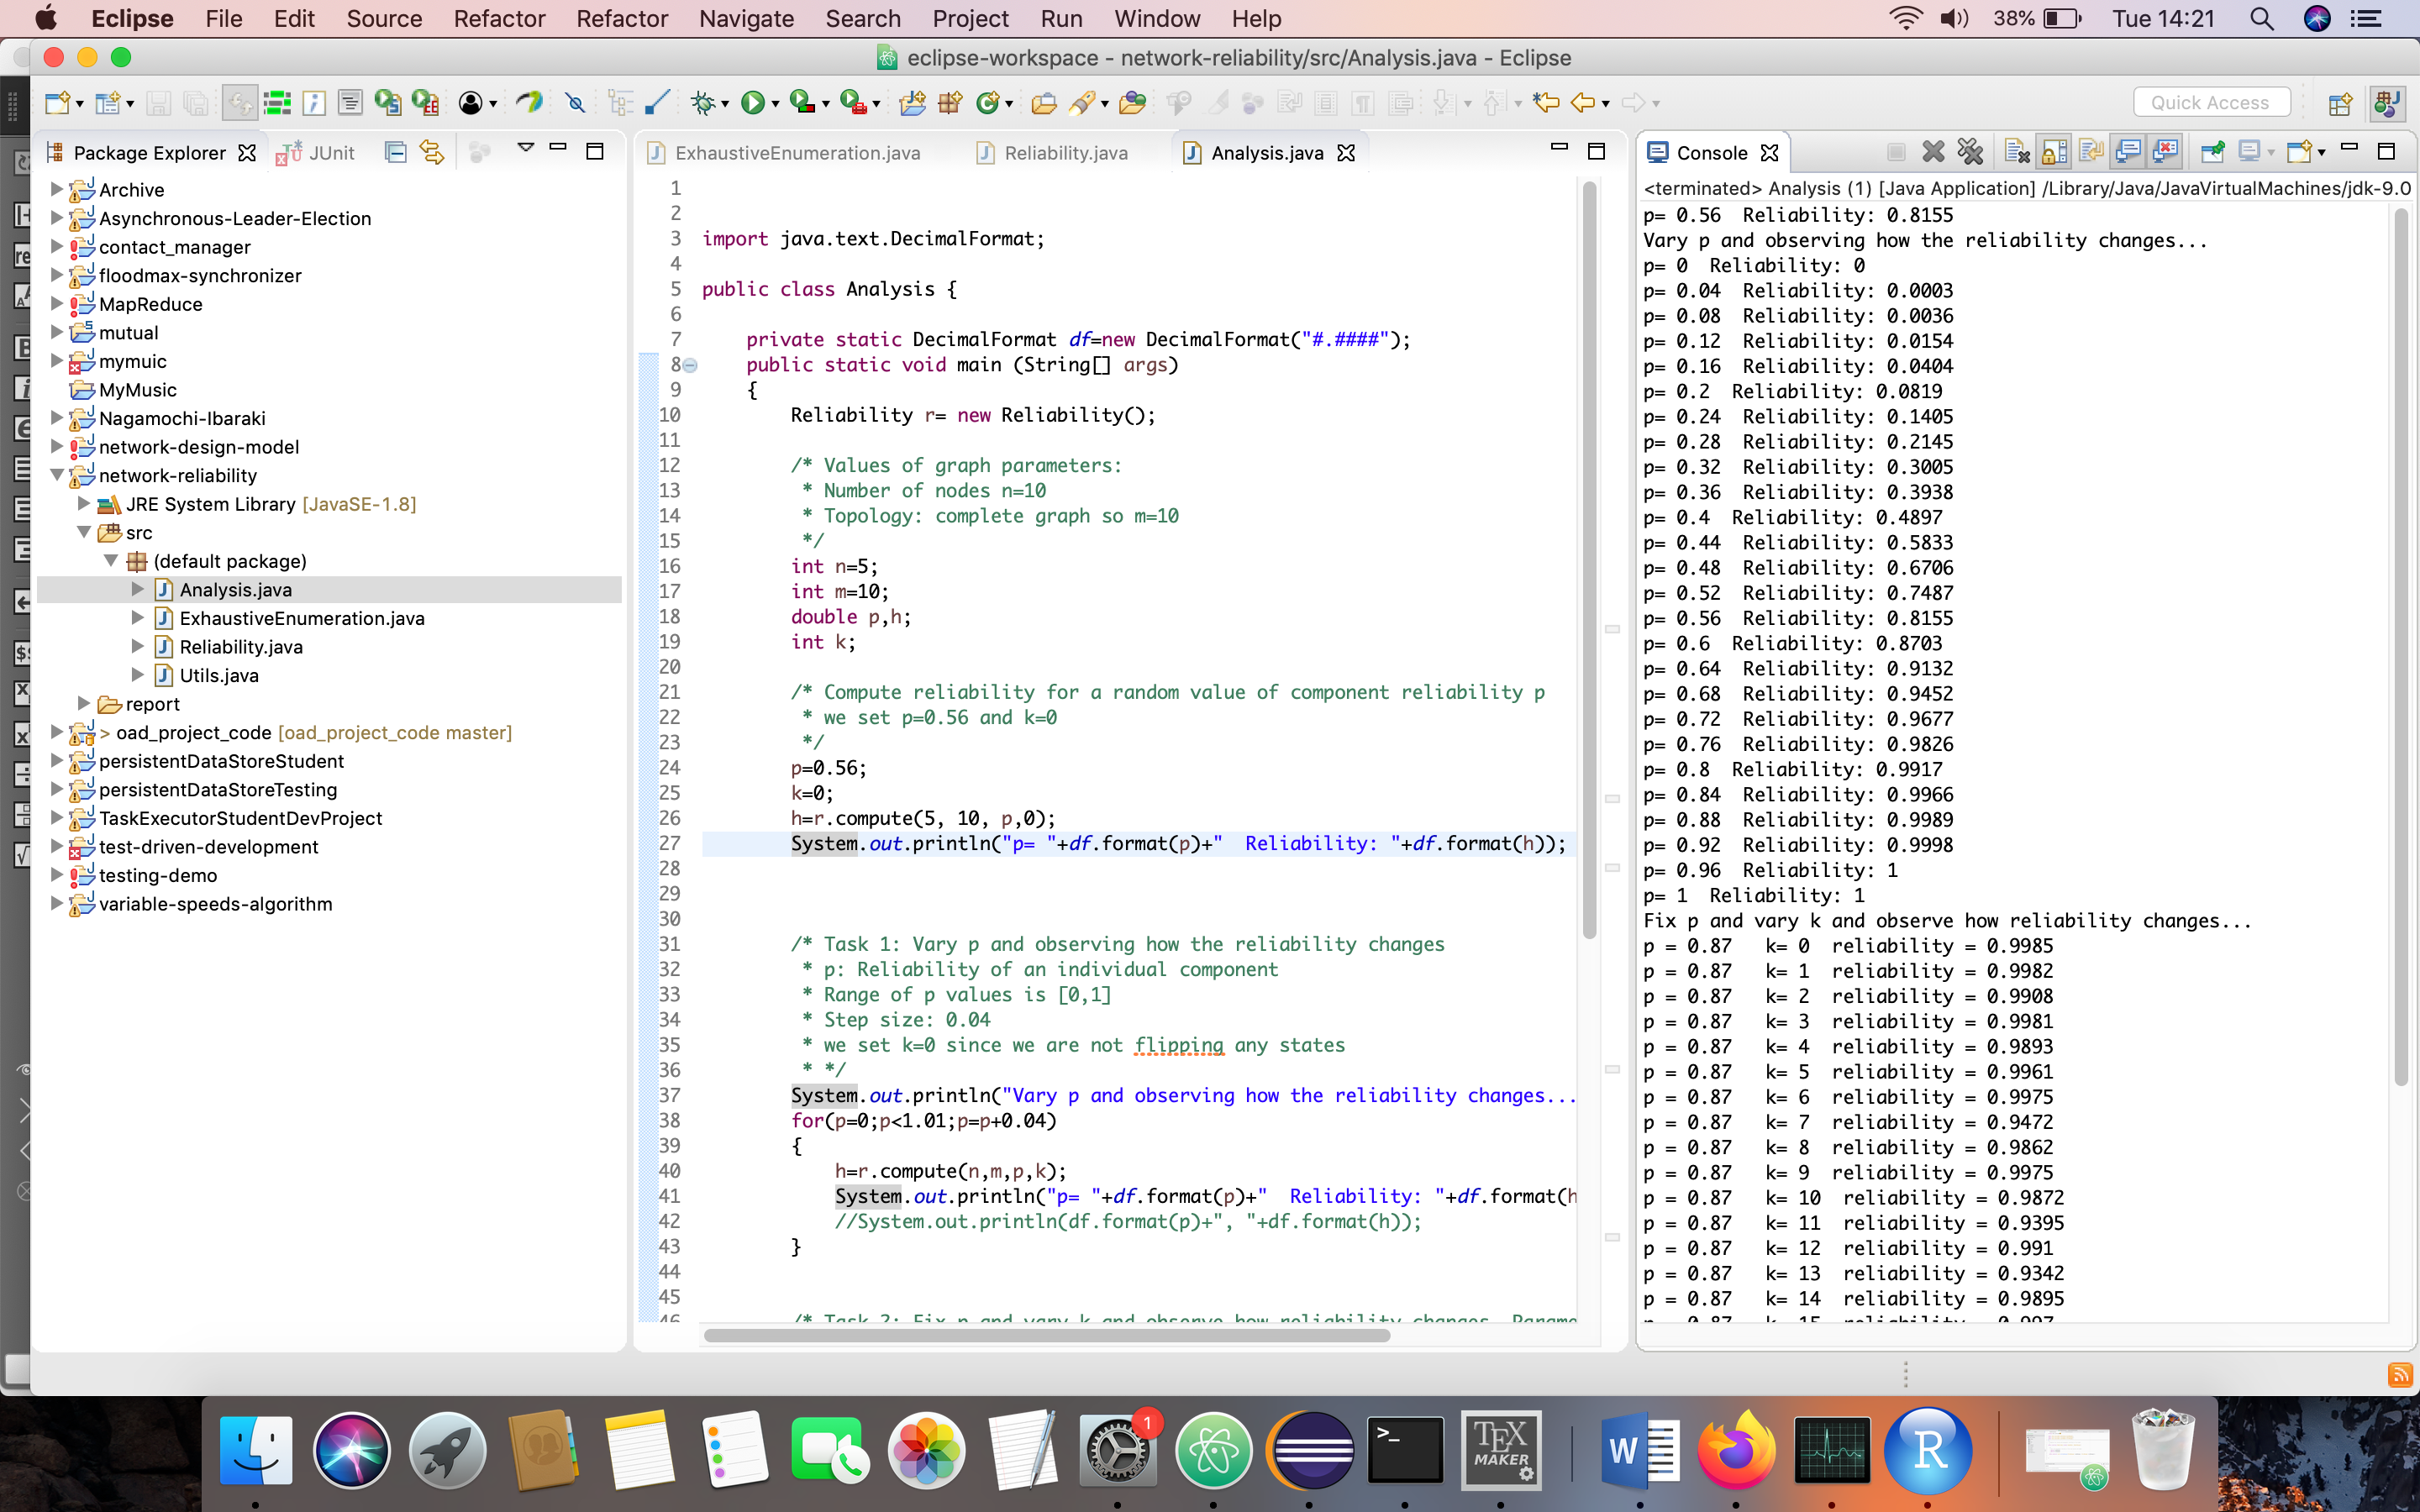
\includegraphics[scale=0.3]{fig/photo1.png}\\

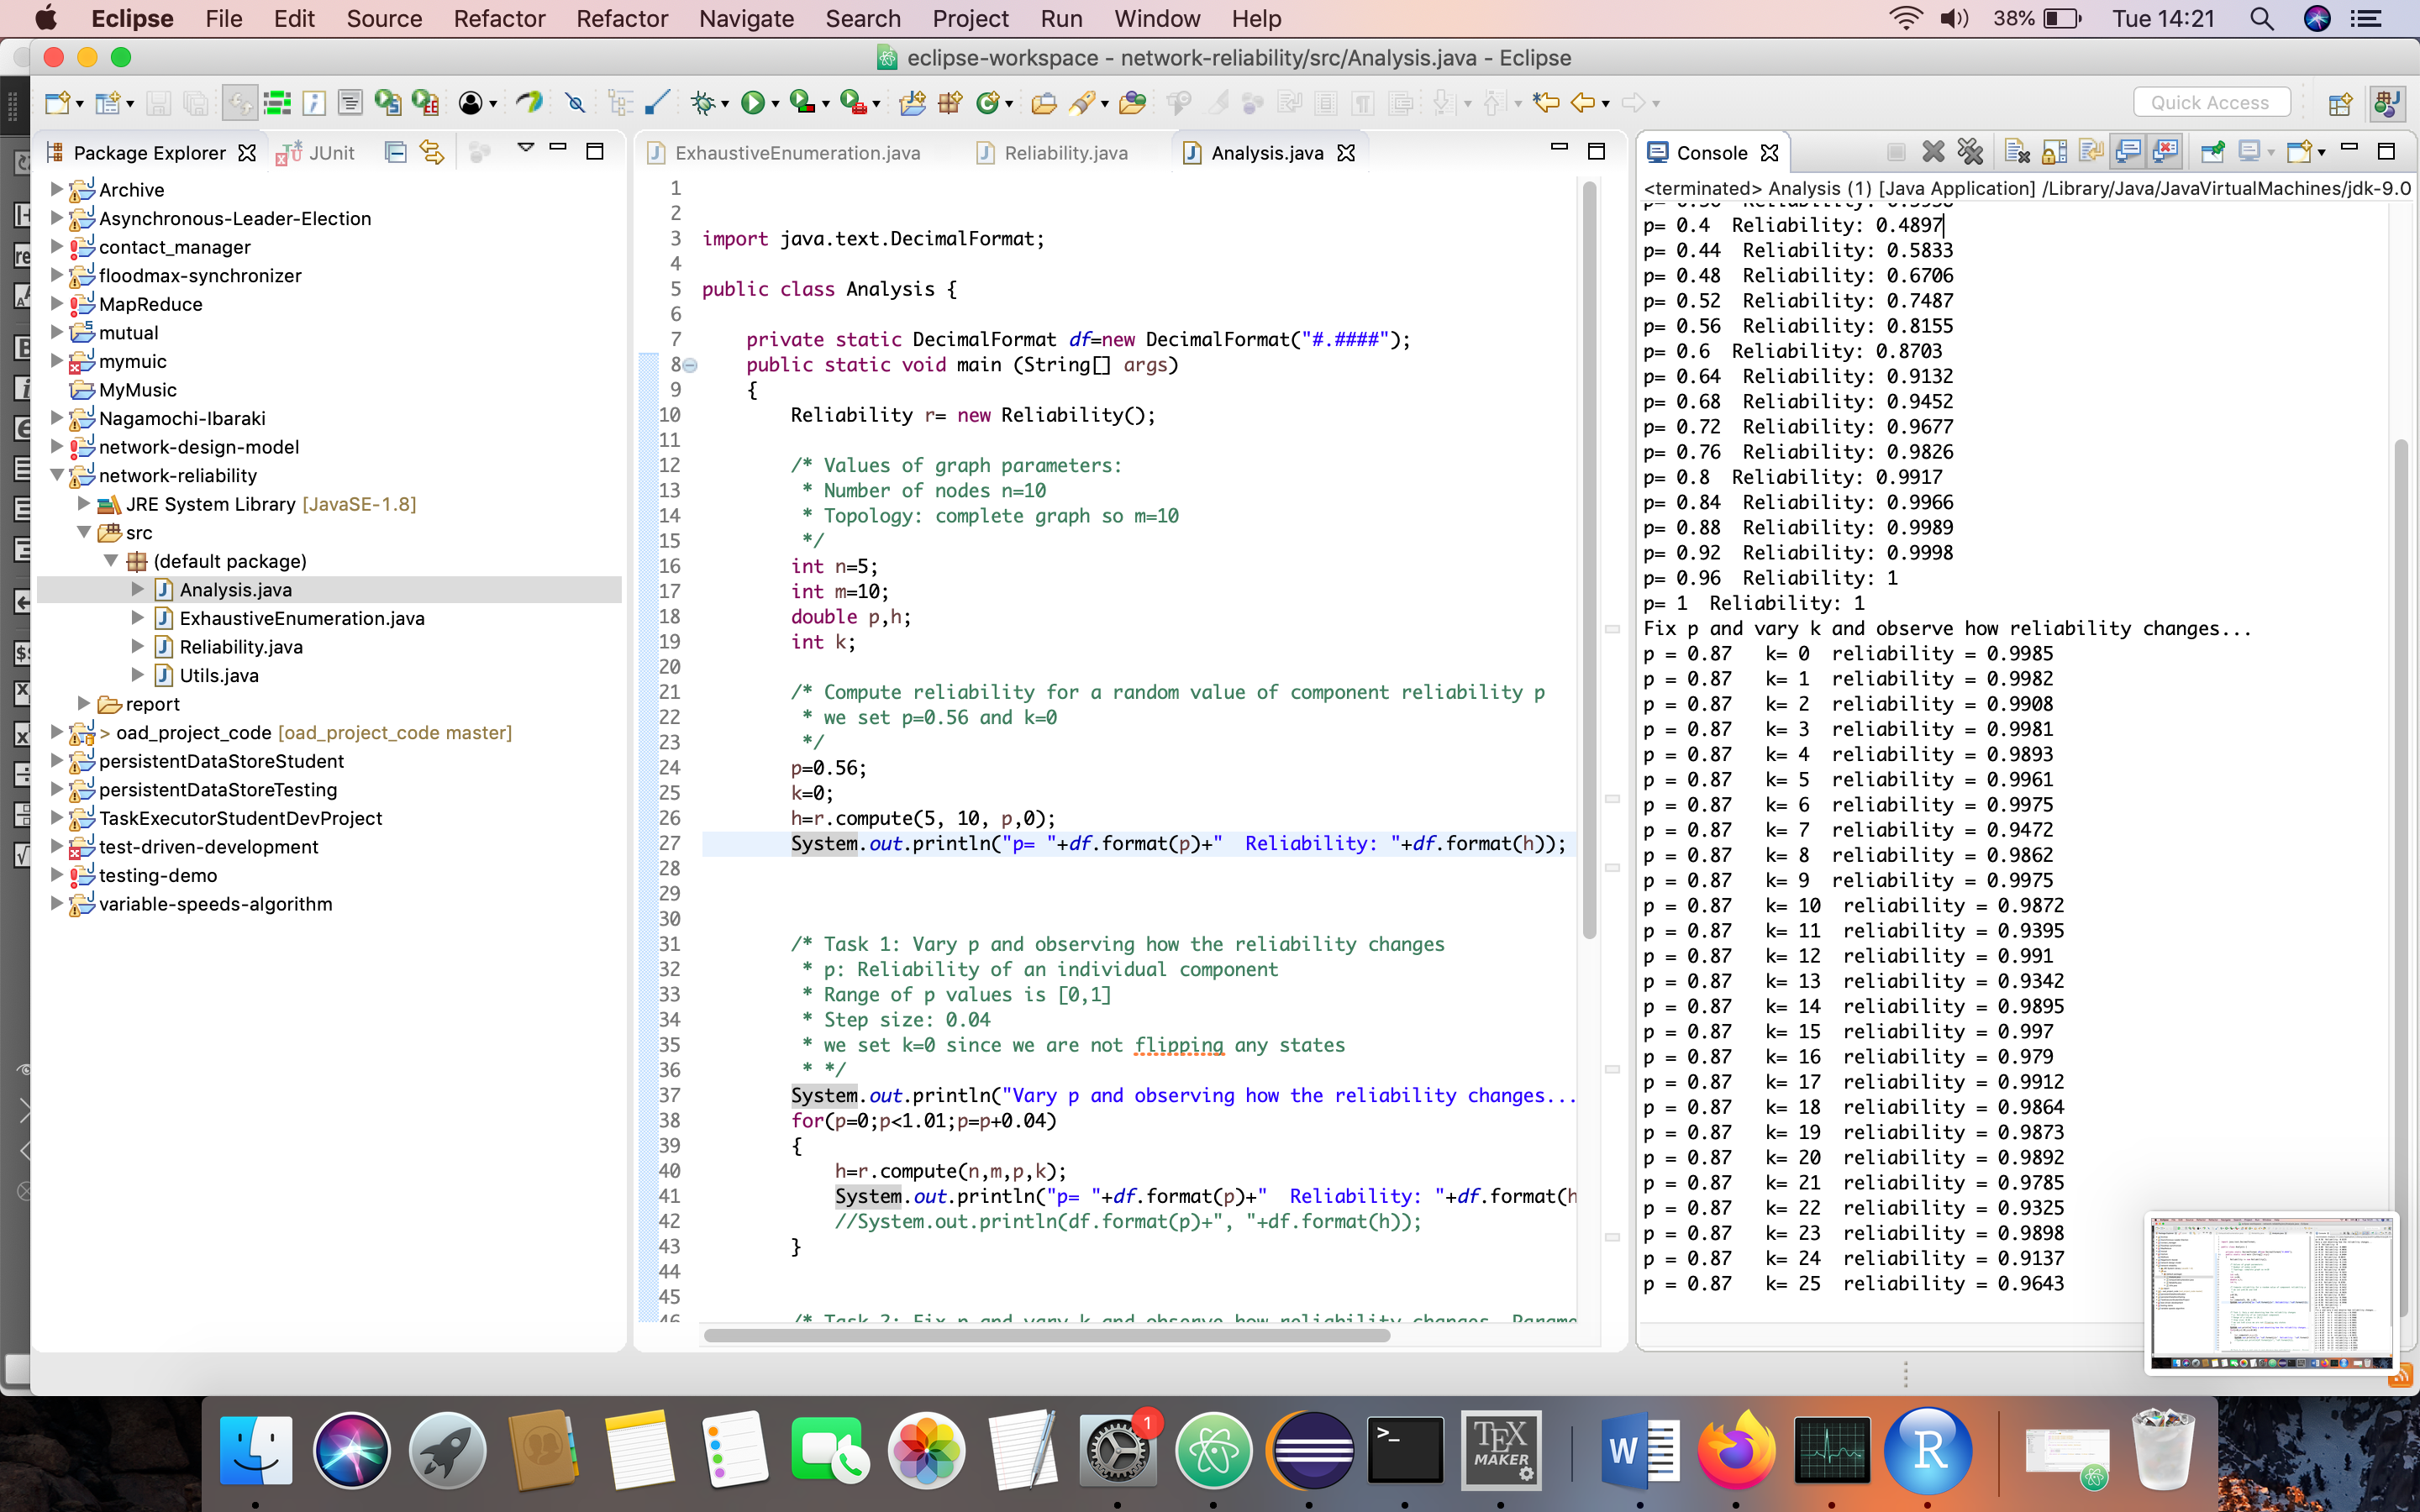
\includegraphics[scale=0.3]{fig/photo2.png}\\

 
\item The output results are stored in a \textit{csv} file. The graphs are generated in \textbf{R}.

\item We plot the graph of the \textit{component reliability} p vs. the \textit{network reliability}. 

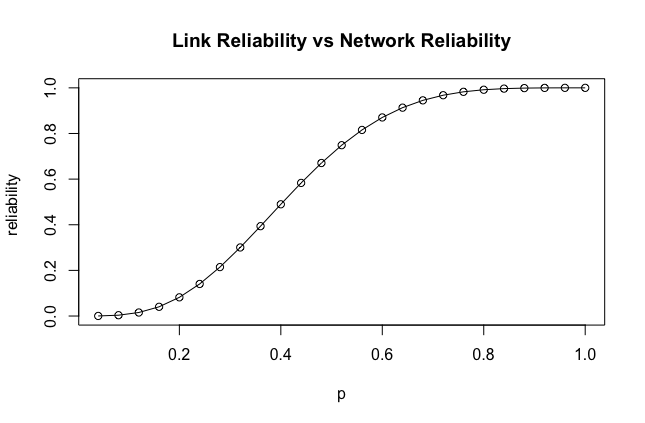
\includegraphics[scale=0.6]{fig/plot1.png}\\

\item We can clearly see that the reliability of the network \textbf{increases} with increase in the value of p



\item We plot the graph of k values  against  network reliabilities.\\

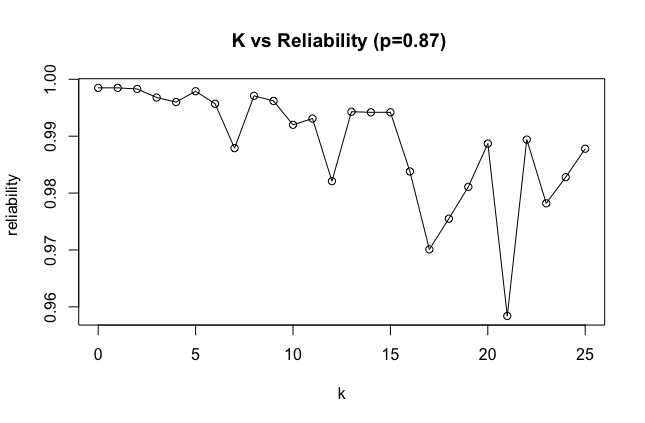
\includegraphics[scale=0.6]{fig/plot2.png}




\item We can clearly see that the reliability of a network shows \textbf{no distinct behaviour} with respect to the k values
\end{itemize}
 
\section{Discussion}
\begin{itemize}

\item As the component reliability \textbf{p} in the graph increases, the probabilities contribution of the \textit{up} states to the network reliability tends to increase, hence the reliability of the graph also \textbf{increases}

\item When we fix the value of p to \textbf{0.87} and \textbf{vary k}, the reliability of the network shows no distinct behavior. Most of the reliability values are close to the reliability value without flipping any states i.e. k=0

\item The reason is that flipping a few states (in our case, a maximum of 25 states out of 1024) does not affect the reliability of the network. This shows that the Exhaustive Enumeration algorithm gives us an accurate estimate of the network reliability even if some states are wrongly assigned system condition.


\end{itemize}





  \section{ReadMe File}
  This section shows how to run the project files.
  \begin{itemize}
  \item Downloads the project files and store them in a folder
  \item Open the project folder in Eclipse
  \item Open the file \textbf{Analysis.java}
  \item Right Click $->$ Run as $->$ Java Application
  \item Alternatively,navigate to the folder in \textbf{terminal} and run the following commands
  \begin{itemize}
  \item javac Analysis.java
  \item java Analysis
  \end{itemize}
  \end{itemize}

  

 
\section{Code}

\textbf{Module 1: ExhaustiveEnumeration.java}
\lstinputlisting{/users/psprao/eclipse-workspace/network-reliability/src/ExhaustiveEnumeration.java}

\pagebreak
\textbf{Module 2: Reliability.java}
\lstinputlisting{/users/psprao/eclipse-workspace/network-reliability/src/Reliability.java}

\pagebreak
\textbf{Module 3: Presentation.java}
\lstinputlisting{/users/psprao/eclipse-workspace/network-reliability/src/Analysis.java}

\pagebreak
\textbf{Utils.java}
\lstinputlisting{/users/psprao/eclipse-workspace/network-reliability/src/Utils.java}



\textbf{Visualization.R.java}
\lstinputlisting{/users/psprao/eclipse-workspace/network-reliability/visualization.R}





\end{document}
